\documentclass{standalone}
\usepackage{pgfplots}
\usepackage{pgfplotstable}
\usepackage{amsmath}

\begin{document}
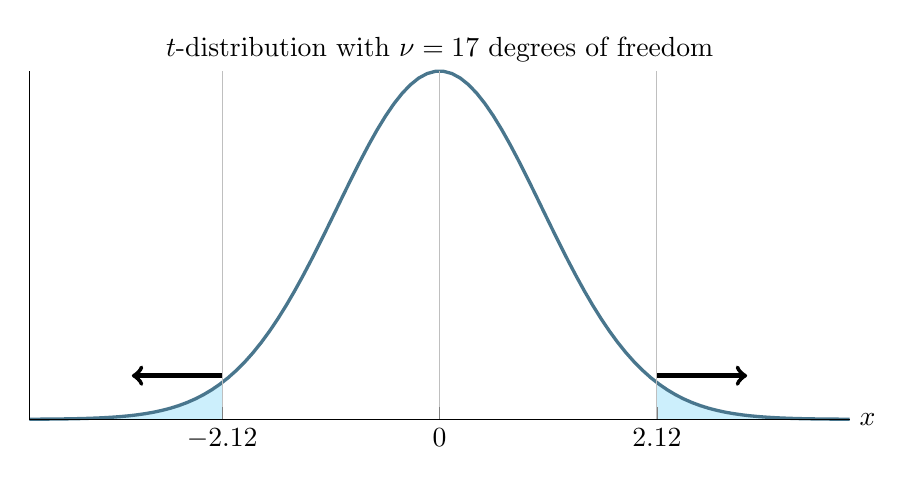
\begin{tikzpicture}
\begin{axis}[
    no markers, domain=-4:4, samples=100,
    axis lines*=left, xlabel=$x$, ylabel={$t$-distribution with $ \nu = 17 $ degrees of freedom},
    every axis y label/.style={at=(current axis.above origin),anchor=south},
    every axis x label/.style={at=(current axis.right of origin),anchor=west},
    height=6cm, width=12cm,
    xtick={-2.12,0,2.12}, ytick=\empty,
    enlargelimits=false, clip=false, axis on top,
    grid = major
]
\addplot [fill=cyan!20, draw=none, domain=-4:-2.12] {exp(-x^2/2)/sqrt(2*pi)} \closedcycle;
\addplot [fill=cyan!20, draw=none, domain=2.12:4] {exp(-x^2/2)/sqrt(2*pi)} \closedcycle;
\addplot [very thick,cyan!50!black] {exp(-x^2/2)/sqrt(2*pi)};

% Add arrows
\draw [->, ultra thick] (axis cs: -2.12,0.05) -- (axis cs: -3,0.05);
\draw [->, ultra thick] (axis cs: 2.12,0.05) -- (axis cs: 3,0.05);
\end{axis}
\end{tikzpicture}
\end{document}
